\documentclass[a4paper,12pt]{article}

\usepackage{amssymb,amsmath}
\usepackage[brazilian]{babel}
\usepackage[utf8]{inputenc}
\usepackage{graphicx}
\usepackage{chngcntr}
\usepackage{tikz}
\usepackage{tikz-3dplot}
\usepackage{indentfirst}
\usepackage[numbers,sort&compress]{natbib}
\usepackage[title]{appendix}
\usepackage{subfig}
\usepackage{floatrow}
\usepackage{booktabs}% http://ctan.org/pkg/booktabs
\newcommand{\tabitem}{~~\llap{\textbullet}~~}

\usetikzlibrary{trees}
\usetikzlibrary{decorations.pathmorphing}
\usetikzlibrary{decorations.markings}

\tikzset{
    photon/.style={decorate, decoration={snake}, draw=black},
    fermion/.style={draw=black, postaction={decorate}, 
    decoration={markings,mark=at position .55 with {\arrow[scale=2,draw=black]{>}}}},
    afermion/.style={draw=black, postaction={decorate}, 
    decoration={markings,mark=at position .55 with {\arrow[scale=2,draw=black]{<}}}},
    gluon/.style={decorate, draw=green,
    decoration={coil,amplitude=4pt, segment length=5pt}} 
    }

\counterwithin{figure}{subsection}

\usepackage{afterpage}

\newcommand\blankpage{%
    \null
    \thispagestyle{empty}%
    \addtocounter{page}{-1}%
    \newpage}
    
\setlength{\parindent}{20pt}


\renewcommand{\and}{\\}
%opening
\title{Equação Qualquer}
%\author{Fabio de Moraes Canedo \and
%7994642}

\begin{document}

\maketitle

\begin{equation*}
\oint_{\partial S} \overrightarrow{D}(\gamma) \cdot d\overrightarrow{\gamma} = \int \int_{S} ( \triangledown\times D) \cdot d \overrightarrow{n}
\end{equation*}

\begin{equation*}
\widehat{f}(k) = \int_{-\infty}^{+\infty} f(x) e^{-ikx} dx
\end{equation*}

\begin{equation*}
z_g = \frac{\min (p_{T,1},p_{T,2})}{p_{T,1}+p_{T,2}}
\end{equation*}

%\begin{abstract}
%A proposta descrita nesse projeto é a de realizar estudos a respeito da fase da matéria conhecida
como plasma de quarks e gluons(\emph{quark-gluon plasma}-QGP) através de observáveis que se relacionam
com quarks pesados(\emph{charm} e \emph{beauty}). Os observáveis visados nesse trabalho referem-se
à estrutura interna de jatos pesados. Especificamente, testaremos modelos diferentes para a geração
de eventos e estudaremos funções de fragmentação através da distribuição angular e energética de subjatos.
%\end{abstract}

%%Arquivo teste para imagens

\begin{figure}
 \begin{center}
 %\tdplotsetmaincoords{70}{120}
 %[tdplot_main_coords, scale=1]

 \begin{tikzpicture}[
        thick,
        % Set the overall layout of the tree
        level/.style={level distance=1.5cm},
        level 2/.style={sibling distance=2.6cm},
        level 3/.style={sibling distance=2cm}
    ]
    \coordinate
        child[grow=left, level distance=0pt]{
            child {
                node {$g$}
                % The 'edge from parent' is actually not needed because it is
                % implicitly added.
                edge from parent [gluon]
            }
            child {
                node {$g$}
                edge from parent [gluon]
            }
        }
        % I have to insert a dummy child to get the tree to grow
        % correctly to the right.
        child[grow=right, level distance=0pt]{
	  child {
	    node {$g$}
	      edge from parent [gluon]
	  }
	  child {
	  node {$g$}
										edge from parent [gluon]
		}
								};
						\end{tikzpicture}

\caption{Tikzpicture}
\label{Tikzpicture}

 \end{center}

\end{figure}

%\section{P1}

%Estudamos aqui o caso do qutrit. Trata-se de um sistema com três estados de energia, a saber:

\begin{equation}
\begin{split}
E_1 & =0 \\
E_2 & =\epsilon+\Delta \\
E_2 & =\epsilon-\Delta
\end{split}
\end{equation}

A quantidade mais importante para estudar as propriedades de equilíbrio desse sistema é 
a função de equipartição, definida por:

\begin{equation}
Z=\sum_i e^{-\beta E_i}
\end{equation}

A partir dessa, todas as outras quantidades de interesse podem ser extraídas. Aplicando, então, as energias supramencionadas, obtemos:

\begin{equation}
Z=1+2e^{-\beta \epsilon}\cosh(\beta \Delta)
\end{equation}

Um plot dessa função pode ser observada na Figura \ref{Z}

\begin{figure}
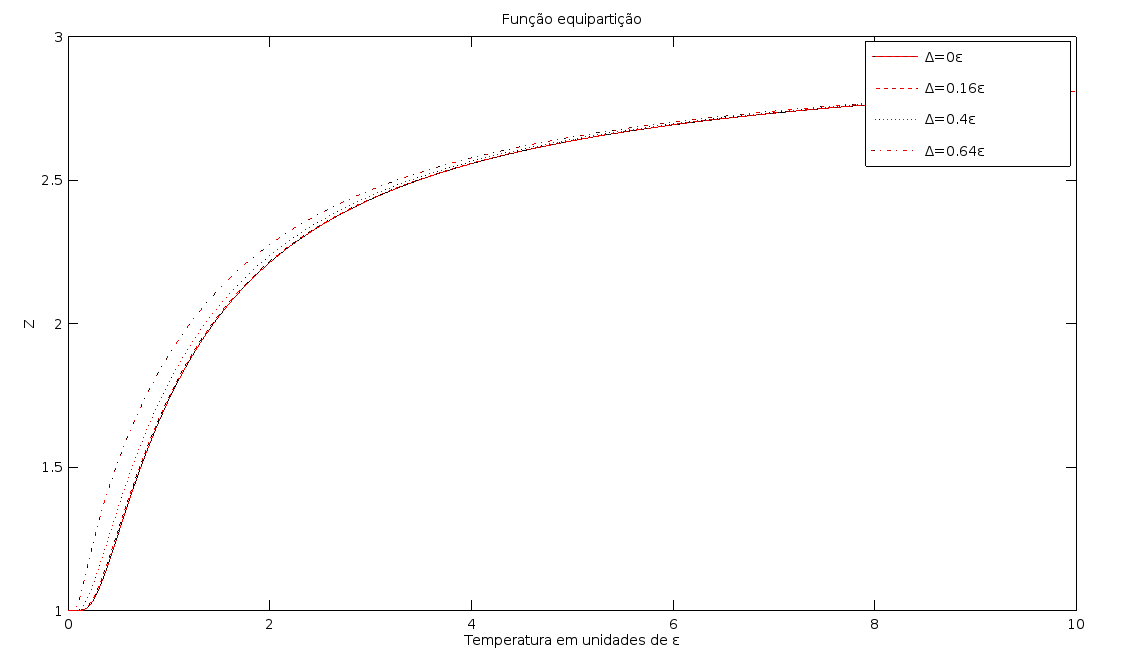
\includegraphics[scale=.3]{Z.png}
\caption{Função equipartição como função da temperatura em unidades de $\epsilon$.}
\label{Z}
\end{figure}

Para obtermos agora, como outras quantidades termodinâmicas se comportam, utilizamos, por exemplo, a identidade:

\begin{equation}
U=-\frac{\partial \ln Z}{\partial \beta}
\end{equation}

De onde podemos obter:

\begin{equation}
U=\frac{2(\epsilon \cosh(\beta \Delta) - \Delta \sinh(\beta \Delta))}{e^{\beta \epsilon} + 2 \cosh(\beta \Delta)}
\end{equation}

A forma dessa função, a chamada energia interna, pode ser observada na Figura \ref{U}

\begin{figure}[!h]
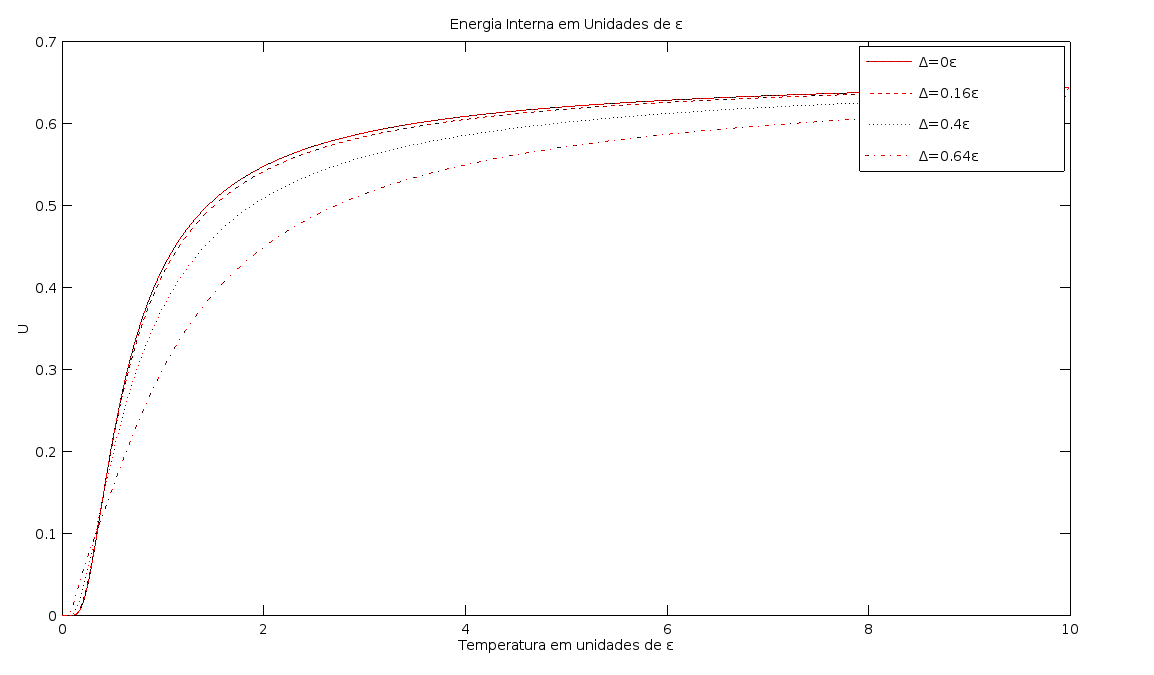
\includegraphics[scale=.3]{U0a10}
\caption{Energia Interna como função da temperatura do sistema calculada em unidades de $\epsilon$.}
\label{U}
\end{figure}

A partir da energia interna, é possível obter também a capacidade térmica:

\begin{equation}
C=\frac{2 \beta^2 \left(e^{\beta \epsilon} \left(\left(\Delta^2+e^2\right) \cosh (\beta \Delta)-2 \Delta \epsilon \sinh (\beta \Delta)\right)+2 \Delta^2\right)}{\left(2 \cosh (\beta \Delta)+e^{\beta \epsilon}\right)^2}
\end{equation}

A forma dessa última pode ser observada na Figura \ref{C}.

\begin{figure}[!h]
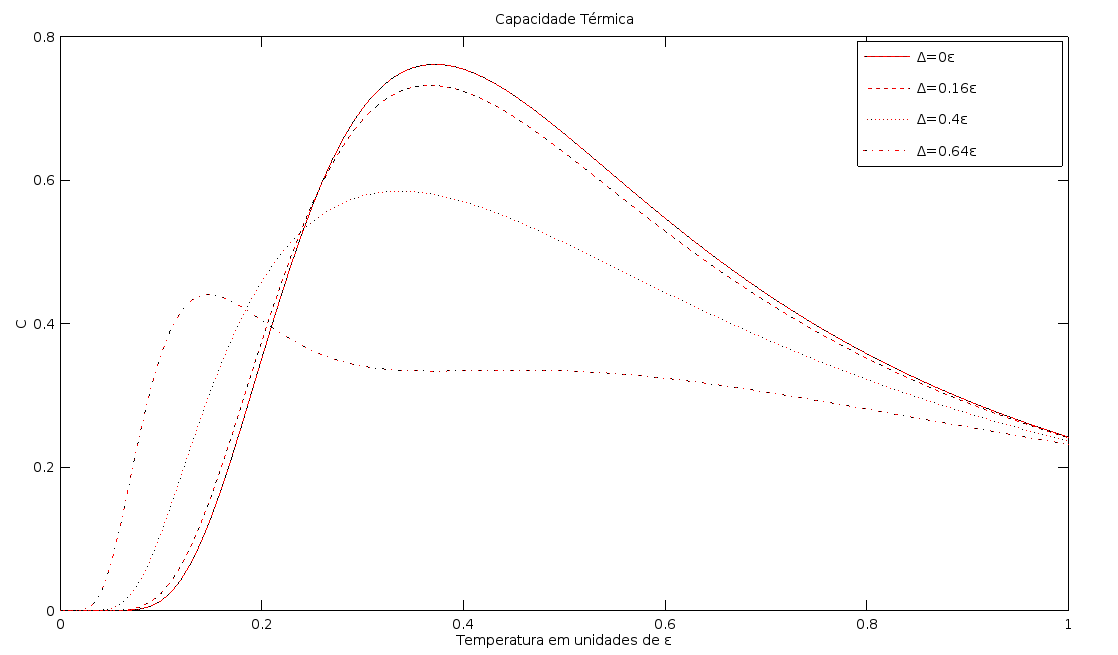
\includegraphics[scale=.3]{Cpeq}
\caption{Capacidade Térmica como função da temperatura do sistema calculada em unidades de $\epsilon$.}
\label{C}
\end{figure}

Para $T \rightarrow \infty$, teremos a capacidade térmica indo para zero. Isso está consistente com as características do sistema, para ilustrar esse ponto, basta pensarmos nas probabilidades de ocupação de cada estado, definidas por:

\begin{equation}
P_i=\frac{e^{-\beta E_i}}{Z}
\end{equation}

Como $T \rightarrow \infty \Rightarrow \beta \rightarrow 0$, teremos todas as probabilidades iguais a $\frac{1}{Z}$, isso resulta em estados equiprováveis e a uma energia igual à média das energias dos estados. Isso implica que a energia interna tem um limite finito bem definido, portanto, fica cada vez mais difícil acrescentar energia no sistema, de maneira que a capacidade térmica tende a zero.

\par

Outras duas quantidades de interesse a ser calculadas são a enerfia livre de Helmholtz e a entropia do sistema, $F$ e $S$, respectivamente. Estas são dadas pelas expressões:

\begin{equation}
\begin{split}
F & = \frac{\ln(Z)}{\beta} \\
S & = \beta(U + F)
\end{split}
\end{equation}

Ambas estão plotadas nas Figuras \ref{F} e \ref{S}.

\begin{figure}[!h]
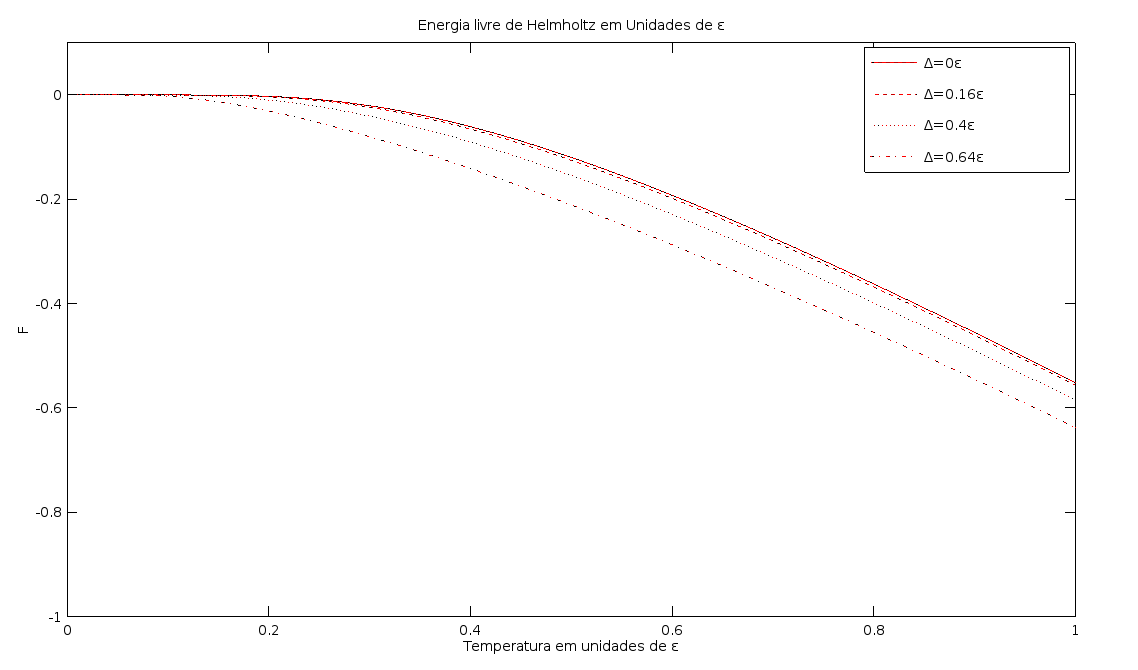
\includegraphics[scale=.3]{F0a1}
\caption{Energia Livre de Helmholtz como função da temperatura do sistema calculada em unidades de $\epsilon$.}
\label{F}
\end{figure}

\begin{figure}[!h]
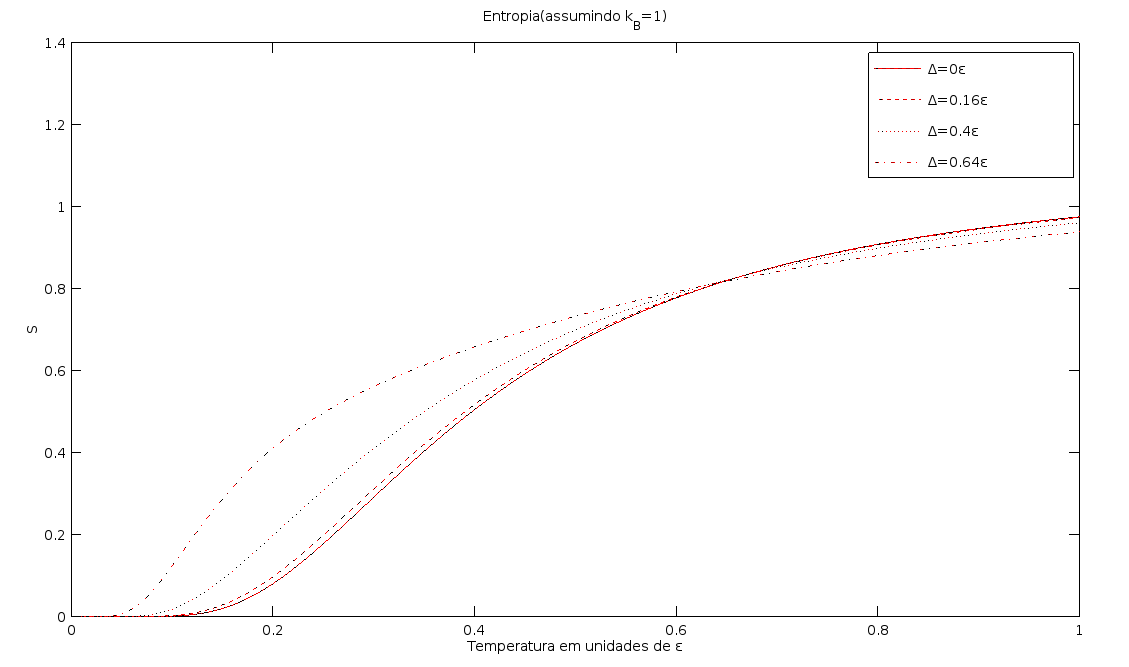
\includegraphics[scale=.3]{entropy}
\caption{Entropia como função da temperatura do sistema calculada em unidades de $\epsilon$.}
\label{S}
\end{figure}

É interessante notar que, para valores mais altos de $\Delta$, a entropia possui um pico que fica maior e se desloca para a esquerda. Para $\Delta=\epsilon$ a entropia do sistema à temperatura zero na realidade é diferente de 0. Isso ocorre porque, nesse caso, o estado fundamental é degenerado e teremos $P_1=P_3=0.5$ e zero para o outro estado. Utilizando a definição de entropia:

\begin{equation}
S=-\sum_i P_i \ln P_i
\end{equation}

Portanto, para $T \rightarrow 0$, teremos $S\rightarrow\ln(2)$

%\section{P2}

%Para esse problema, teremos uma Hamiltoniana definida por:

\begin{equation}
H=kS_{x}^{2} + \lambda S_z
\end{equation}

Onde:

\begin{equation}
Sx=\left(
\begin{array}{ccc}
 0 & \frac{1}{\sqrt{2}} & 0 \\
 \frac{1}{\sqrt{2}} & 0 & \frac{1}{\sqrt{2}} \\
 0 & \frac{1}{\sqrt{2}} & 0 \\
\end{array}
\right),
Sz= \left(
\begin{array}{ccc}
 1 & 0 & 0 \\
 0 & 0 & 0 \\
 0 & 0 & -1 \\
\end{array}
\right)
\end{equation}

A Hamiltoniana escrita em forma de matriz fica então:

\begin{equation}
H= \left(
\begin{array}{ccc}
 \lambda & \frac{k}{2} & 0 \\
 \frac{k}{2} & 0 & \frac{k}{2} \\
 0 & \frac{k}{2} & -\lambda \\
\end{array}
\right)
\end{equation}

Os autovalores podem ser achados pelas raízes do polinômio característico, e serão:

\begin{equation}
\begin{split}
E_1&=0 \\
E_2&=-\sqrt{\frac{k^2}{2}+\lambda^2} \\
E_3&=\sqrt{\frac{k^2}{2}+\lambda^2}
\end{split}
\end{equation}





%\bibliography{Bibliografia/bibliografia} 
%\bibliographystyle{IEEEtran}
%\bibliographystyle{ieeetr}

\end{document}